
%(BEGIN_QUESTION)
% Copyright 2006, Tony R. Kuphaldt, released under the Creative Commons Attribution License (v 1.0)
% This means you may do almost anything with this work of mine, so long as you give me proper credit

Noen bourdon-rorsmanometre er utstyrt med en veldig liten spiralfjær festet til viserakselen:

$$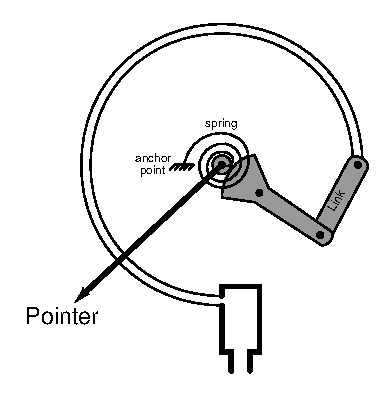
\includegraphics[width=15.5cm]{i00175x01.eps}$$

Denne fjæren er for svak til å ha noen målbar effekt på span i instrumentet.  Med andre ord motvirker den ikke bøyningen i bourdon-røret i målbar grad, slik en ``range spring'' ville gjort i andre instrumentdesign.

Gitt at den er så svak, hvilken funksjon kan denne fjæren ha i manometermekanismen?

\vskip 10pt

\underbar{file i00175}
%(END_QUESTION)





%(BEGIN_ANSWER)

Dette er en ``anti-backlash''-fjær som gir nok moment til å fjerne ``slakk'' i sektor/pinjong-tannhjulene, slik at viseren alltid reagerer på de minste endringer i bourdon-rorets posisjon.

%(END_ANSWER)





%(BEGIN_NOTES)

En annen metode for å eliminere backlash i tannhjulsinstrumenter er å bruke to sideplasserte tannhjul som spennes av en spiralfjær, der begge griper i ett felles drivhjul.  Med to tannhjul som griper mot ett og med motsatt moment i de to tannhjulene, blir det ingen ``løshet'' i transmisjonen som kan skape dødband eller hysterese i viserbevegelsen.

Hvis helt backlash-fri bevegelsesoverføring ønskes, kan tannhjul erstattes av hjul koblet med bånd av fjærstål i en presisjonsmekanisme.  Slike drivkoblinger brukes ofte i posisjoneringsmekanismer for lesehoder i harddisker.  Ideen med å bruke et fleksibelt metallband som backlash-fri kobling er ikke unik for rotasjonsbevegelse: brukt som små-vinkel-pivot kalles slike bånd \textit{flexures}.

%INDEX% Measurement, pressure: bourdon tube (anti-backlash spring)

%(END_NOTES)
